\documentclass[12pt]{article}
\usepackage[pdftex]{graphicx}
\usepackage[margin=.5in]{geometry}

\renewcommand{\baselinestretch}{1}
\begin{document}
\title{Likelihood Surface Using Different Seeds}

\author{Siddhartha Shelton}
\maketitle
\setcounter{secnumdepth}{3}
\setcounter{tocdepth}{3}

\section{Plots}
Below are several plots of likelihood surfaces. The sweeps were performed over the Forward Evolve time, the Backward evolve time, the radius of the Baryonic matter, the ratio between the radius of the baryonic to the dark matter component, the mass of the Baryonic and, the ratio between the mass of the Baryonic and dark matter component. Each parameter sweep was performed for two different seeds, 125896 and 491349.

\begin{figure}[h!]
\centering
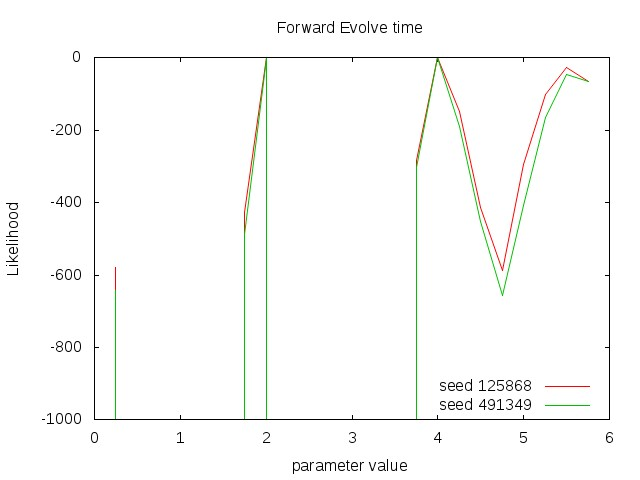
\includegraphics[width=20cm]{./plots/fortime.jpeg}
\caption{Forward time=4 Gyr}
\end{figure}

\begin{figure}[h!]
\centering
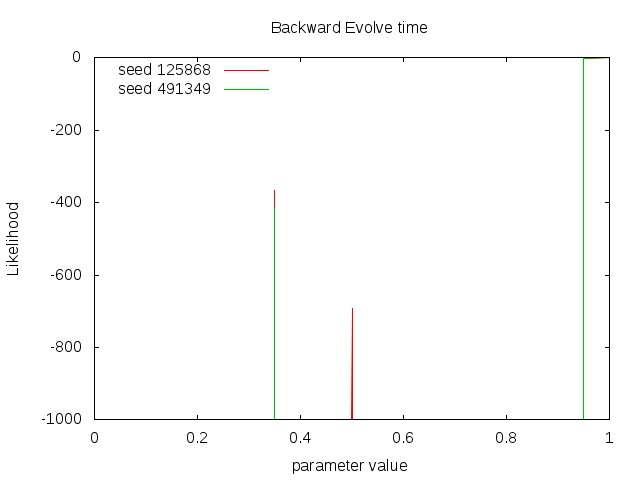
\includegraphics[width=20cm]{./plots/backtime.jpeg}
\caption{Backward Evolve time= 1 Gyr}
\end{figure}

\begin{figure}[h!]
\centering
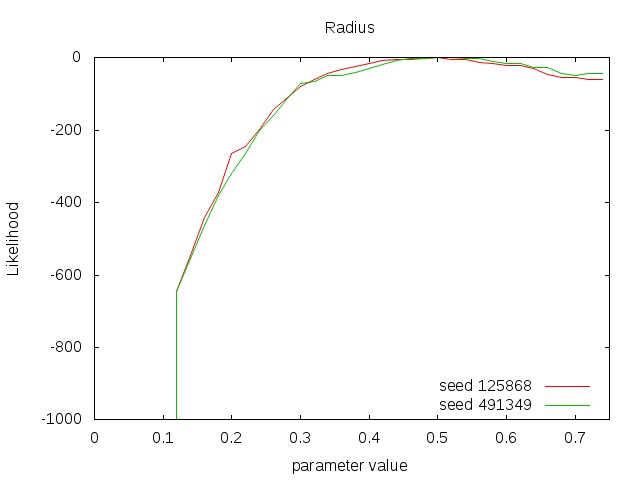
\includegraphics[width=20cm]{./plots/rad.jpeg}
\caption{Radius= 0.5 parsec}
\end{figure}

\begin{figure}[h!]
\centering
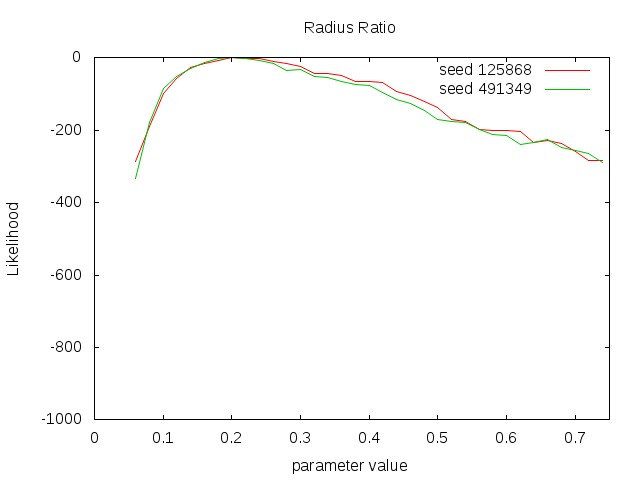
\includegraphics[width=20cm]{./plots/radratio.jpeg}
\caption{Radius ratio= 0.2}
\end{figure}

\begin{figure}[h!]
\centering
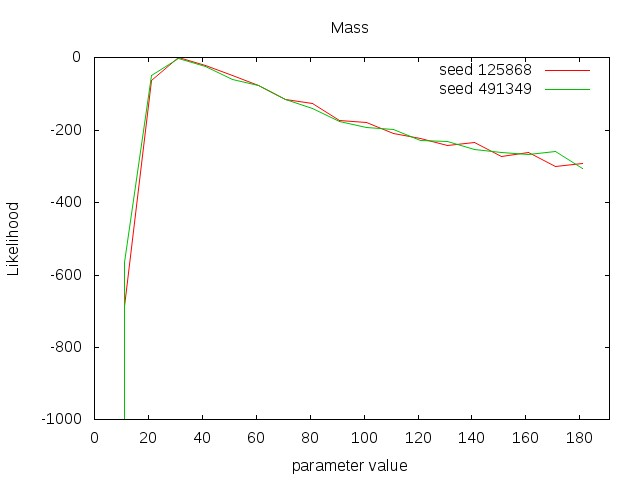
\includegraphics[width=20cm]{./plots/mass.jpeg}
\caption{Mass= 30 simulation masses}
\end{figure}

\begin{figure}[h!]
\centering
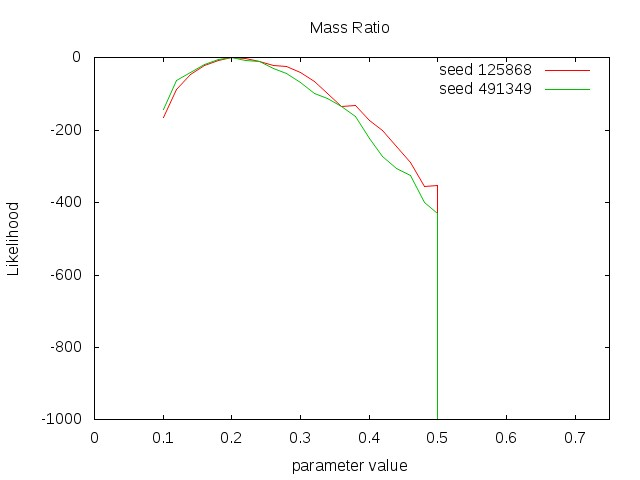
\includegraphics[width=20cm]{./plots/massratio.jpeg}
\caption{Mass ratio= 0.2}
\end{figure}

\end{document}